% !TEX encoding   = UTF8
% !TEX spellcheck = ru_RU
% !TEX root = ../seminars.tex

%%==========================
\chapter{Графические классы}
%%==========================
В~качестве образца приведём несколько примеров решения упражнений. Выполняя некоторые упражнения, мы по~сути расширяем графическую библиотеку, поэтому включим все новые классы в~пространство имён \code{Graph\_lib}. Весь этот код разместим в~каталоге \code{projects/lib/Graph\_lib/ext}. Заголовки и определения классов в~файле \code{graph.h}:

\cppfile[lastline=2, linenos=false]{projects/lib/Graph_lib/ext/graph.h}
\cpp`// ... (standard headers)`
\cppfile[firstline=6, lastline=8, linenos=false]{projects/lib/Graph_lib/ext/graph.h}
\cpp`// ... (extension classes)`
\cppfile[firstline=81, linenos=false]{projects/lib/Graph_lib/ext/graph.h}

\noindent а реализацию функций "--- в~\code{graph.cpp}:

\cpp`// ... (standard headers)`
\cppfile[firstline=4, lastline=6, linenos=false]{projects/lib/Graph_lib/ext/graph.cpp}
\cpp`// ... (methods implementation)`
\cppfile[firstline=187, linenos=false]{projects/lib/Graph_lib/ext/graph.cpp}



%%===================
\section{Дуга (арка)}
%%===================
Рассмотрим класс \code{Arc} для~рисования дуги (или арки) из~упражнения~1 \textbookref{главы~13}. Дуга должна быть частью эллипса. Соответственно, разумно в~качестве базового класса выбрать \code{Ellipse}. Это позволит использовать часть уже разработанной функциональности.

\begin{figure}[ht]
    {\centering
        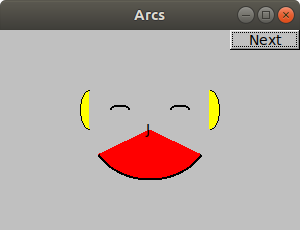
\includegraphics[height=0.25\textwidth]{images/arc.png}~\textit{a})
        \hfil
        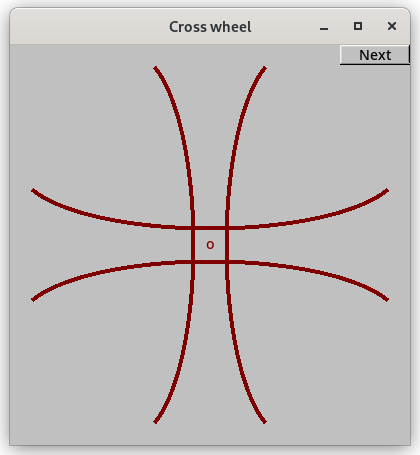
\includegraphics[height=0.25\textwidth]{images/cross_wheel.png}~\textit{б})
        \hfil
        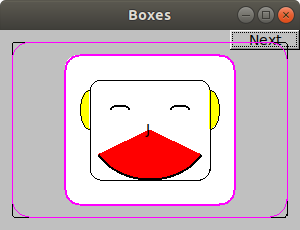
\includegraphics[height=0.25\textwidth]{images/box.png}~\textit{в})

    }
    \caption{Рожицы из~арок и мальтийский крест}
    \label{fig:arc}
\end{figure}

\cppfile[firstline=10, lastline=29]{projects/lib/Graph_lib/ext/graph.h}

\noindent
Ограничений на~начальный и конечный углы дуги мы не~накладываем.

В~конструкторе необходимо инициализировать часть, соответствующую базовому классу \code{Ellipse}, а затем углы, которые мы добавили для~арки:

\cppfile[firstline=8, lastline=11]{projects/lib/Graph_lib/ext/graph.cpp}

В~наиболее сложной части, а именно, отрисовке фигуры, мы взяли за~основу функцию из~класса \code{Ellipse}. Всё, что нужно, "--- это изменить углы:

\cppfile[firstline=13, lastline=26]{projects/lib/Graph_lib/ext/graph.cpp}

Теперь мы можем нарисовать рожицу из~нескольких дуг, используя класс \code{Arc}, например, как показано на~рисунке~\ref{fig:arc}\textit{a}. Нос добавлен при~помощи метки \code{Mark}.



%%============================================
\section{Прямоугольник с~закруглёнными углами}
%%============================================
Теперь рассмотрим класс \code{Box} из~упражнения~2 \textbookref{главы~13}. Он очень похож на~обычный прямоугольник. Единственное, что необходимо добавить, "--- радиус скругления углов. После не~слишком удачной реализации с~хранением четырёх линий в~объекте \code{Lines} и четырёх дуг в~массиве из~объектов \code{Arc}, мы решили наследовать от~\code{Rectangle}:

\cppfile[firstline=32, lastline=51]{projects/lib/Graph_lib/ext/graph.h}

Если пользователь не~указал радиус скругления, мы решили по~умолчанию задать величину 10\,\% от~наименьшей стороны. Это удобно. Но поскольку эта величина известна только на~этапе выполнения, необходим некий трюк. Мы задали в~качестве значения по~умолчанию (константа \code{automatic}) наибольшее целое число, представимое типом \code{int} (необходим заголовок \code{<limits>}).

Реализация первого конструктора довольно проста, отрицательные радиусы скругления мы отбрасываем:

\cppfile[firstline=28, lastline=36]{projects/lib/Graph_lib/ext/graph.cpp}

Второй конструктор совершенно аналогичен. Следует инициализировать базовую часть "--- класс \code{Rectangle} "--- двумя угловыми точками, а для~получения длины и ширины в~теле конструктора можно воспользоваться методами \code{width()} и \code{height()}.

Функция изменения радиуса скругления \code{set\_roundness()} также должна выполнить проверку на~неотрицательность аргумента, после чего присвоить новый радиус.

Стоит уделить внимание отрисовке. Она несколько сложнее, чем для~арки или прямоугольника, особенно, если добавить поддержку заливки фигуры цветом. Код функции представлен ниже:

\cppfile[firstline=47, lastline=54]{projects/lib/Graph_lib/ext/graph.cpp}
\cpp`    // ... use fl_pie() and fl_rectf()`
\cppfile[firstline=67, lastline=83]{projects/lib/Graph_lib/ext/graph.cpp}

Добавим контуры нашей рожице и несколько рамок с~разным скруглением, используя класс \code{Box}, например, как показано на~рисунке~\ref{fig:arc}\textit{в}.



%%================
% !TEX encoding   = UTF8
% !TEX spellcheck = ru_RU
% !TEX root = ../seminars.tex

%%================================
\section{Правильный шестиугольник}
%%================================
Рассмотрим класс \code{Regular\_hexagon} из~упражнения~8 \textbookref{главы~13}. Правильный шестиугольник, по~сути, является многоугольником \code{Polygon}. Однако он не~может содержать количество вершин, отличное от~6-ти. Таким образом, заманчиво наследовать от~\code{Polygon}, но тогда функцию \code{add()}, добавляющую дополнительные точки, необходимо как-то исключить из~интерфейса. И хотя, в~принципе, некоторые языки (с~динамической типизацией) позволяют сделать это, наследование интерфейса нарушилось бы. То есть там, где требуется \code{Polygon} мы не~смогли бы использовать \code{Regular\_hexagon}, в~который нельзя добавлять точки.

Хоть это лишает нас возможности воспользоваться реализацией классов \code{Polygon} или \code{Closed\_polyline}, \emph{логически правильным} решением является наследовать от~абстрактной фигуры \code{Shape}:
\cppfile[firstline=49, lastline=61]{projects/lib/Graph_lib/ext/graph.h}

В~конструкторе добавляем точки, используя вращательную симметрию:
\cppfile[firstline=99, lastline=113]{projects/lib/Graph_lib/ext/graph.cpp}

\noindent Округление при~помощи функции \code{std::round()} вместо отбрасывания дробной части даёт возможность слегка улучшить качество рисования в~отдельных случаях.

В~реализации следующих методов, которые предоставляются для~удобства пользователей, применяется априорное знание об~ориентации шестиугольника на~плоскости:
\cppfile[firstline=115, lastline=133]{projects/lib/Graph_lib/ext/graph.cpp}

Заметим, что эти функции можно было бы вынести из~класса, то есть сделать внешними по~отношению к~классу. Тем не~менее, мы расположили их внутри, поскольку это свойства самих объектов и эти свойства есть у~подобных объектов других типов. Например, у~окна также есть длина (\code{x\_max()}) и ширина (\code{y\_max()}).

Код оставшейся функции \code{draw\_lines()} в~точности повторяет реализацию из~классов \code{Open\_polyline} и \code{Closed\_polyline}:
\cppfile[firstline=135, lastline=157]{projects/lib/Graph_lib/ext/graph.cpp}

Пример рисования правильных шестиугольников показан на~рисунке~\ref{fig:regularhexagon}.



%%==================================
\section{Мозаика из~шестиугольников}
%%==================================
Применим разработанный класс \code{Regular\_hexagon} для~рисования мозаики в~пределах прямоугольной области из~упражнения~9 \textbookref{главы~13}.

\begin{figure}[ht]
  {\centering
    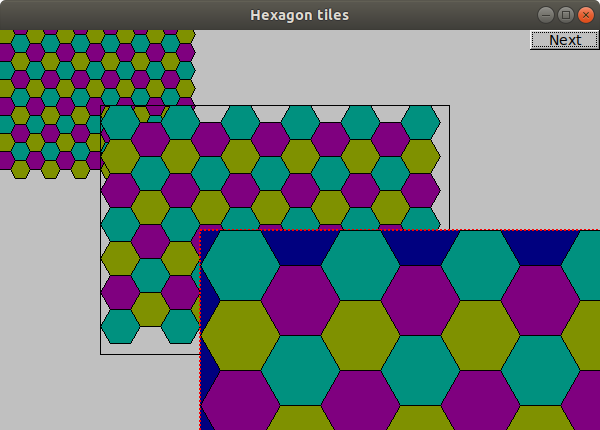
\includegraphics[width=0.6\textwidth]{images/hexagon_tiles.png}

  }
  \caption{Элементы мозаики из~правильных шестиугольников}
  \label{fig:regularhexagon}
\end{figure}

Наследование выполним от~класса \code{Rectangle}, а для~хранения множества правильных шестиугольников воспользуемся классом \code{Vector\_ref}:

\cppfile[firstline=64, lastline=76]{projects/lib/Graph_lib/ext/graph.h}

Вся работа по~формированию мозаики выполняется в~конструкторе. Параметры~\code{p}, \code{ww} и~\code{hh} задают прямоугольник, который заполняется одинаковыми правильными шестиугольниками. Размер шестиугольников определяется радиусом описанной окружности \code{rr}. Код конструктора приведён ниже:

\cppfile[firstline=160, lastline=190]{projects/lib/Graph_lib/ext/graph.cpp}

\begin{figure}[ht]
  {\centering
    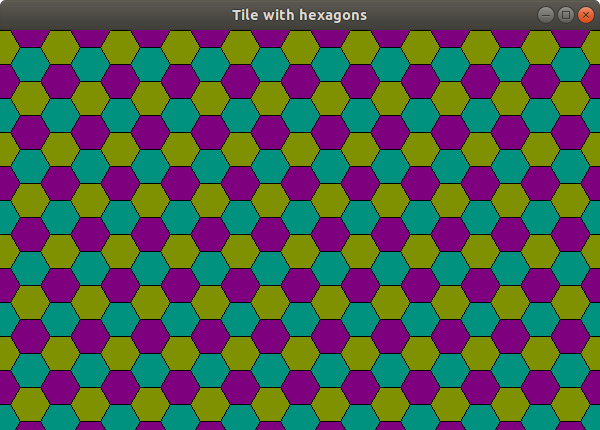
\includegraphics[width=0.6\textwidth]{images/tile_window.png}

  }
  \caption{Окно, полностью заполненное мозаикой}
  \label{fig:hexagontile}
\end{figure}

Реализация перекрывающих методов выполняется тривиально:

\cppfile[firstline=192, lastline=204]{projects/lib/Graph_lib/ext/graph.cpp}

В~начале мы рисуем прямоугольник, затем мозаику. По~умолчанию, прямоугольник не~рисуется. Это поведение мы установили в~конструкторе класса, задав невидимый цвет. Если изменить цвет рисования, то мы увидим границу (и заливку) прямоугольной области, как показано на~рисунке~\ref{fig:regularhexagon}. На~рисунке~\ref{fig:hexagontile} мозаикой покрыта вся область окна.

%%================



%%================
\WhatToReadSection
%%================
\textcite{Stroustrup:2016:ru}: \textbf{глава~14}



%%===============
\ExercisesSection
%%===============
\begin{exercise}
\item Выполните упражнения из~\textbookref{главы~13} учебника.

\begin{figure}[ht]
    {\centering
        \hfill
        \subbottom[Спираль Дюрера\label{fig:spirals:a}]{%
            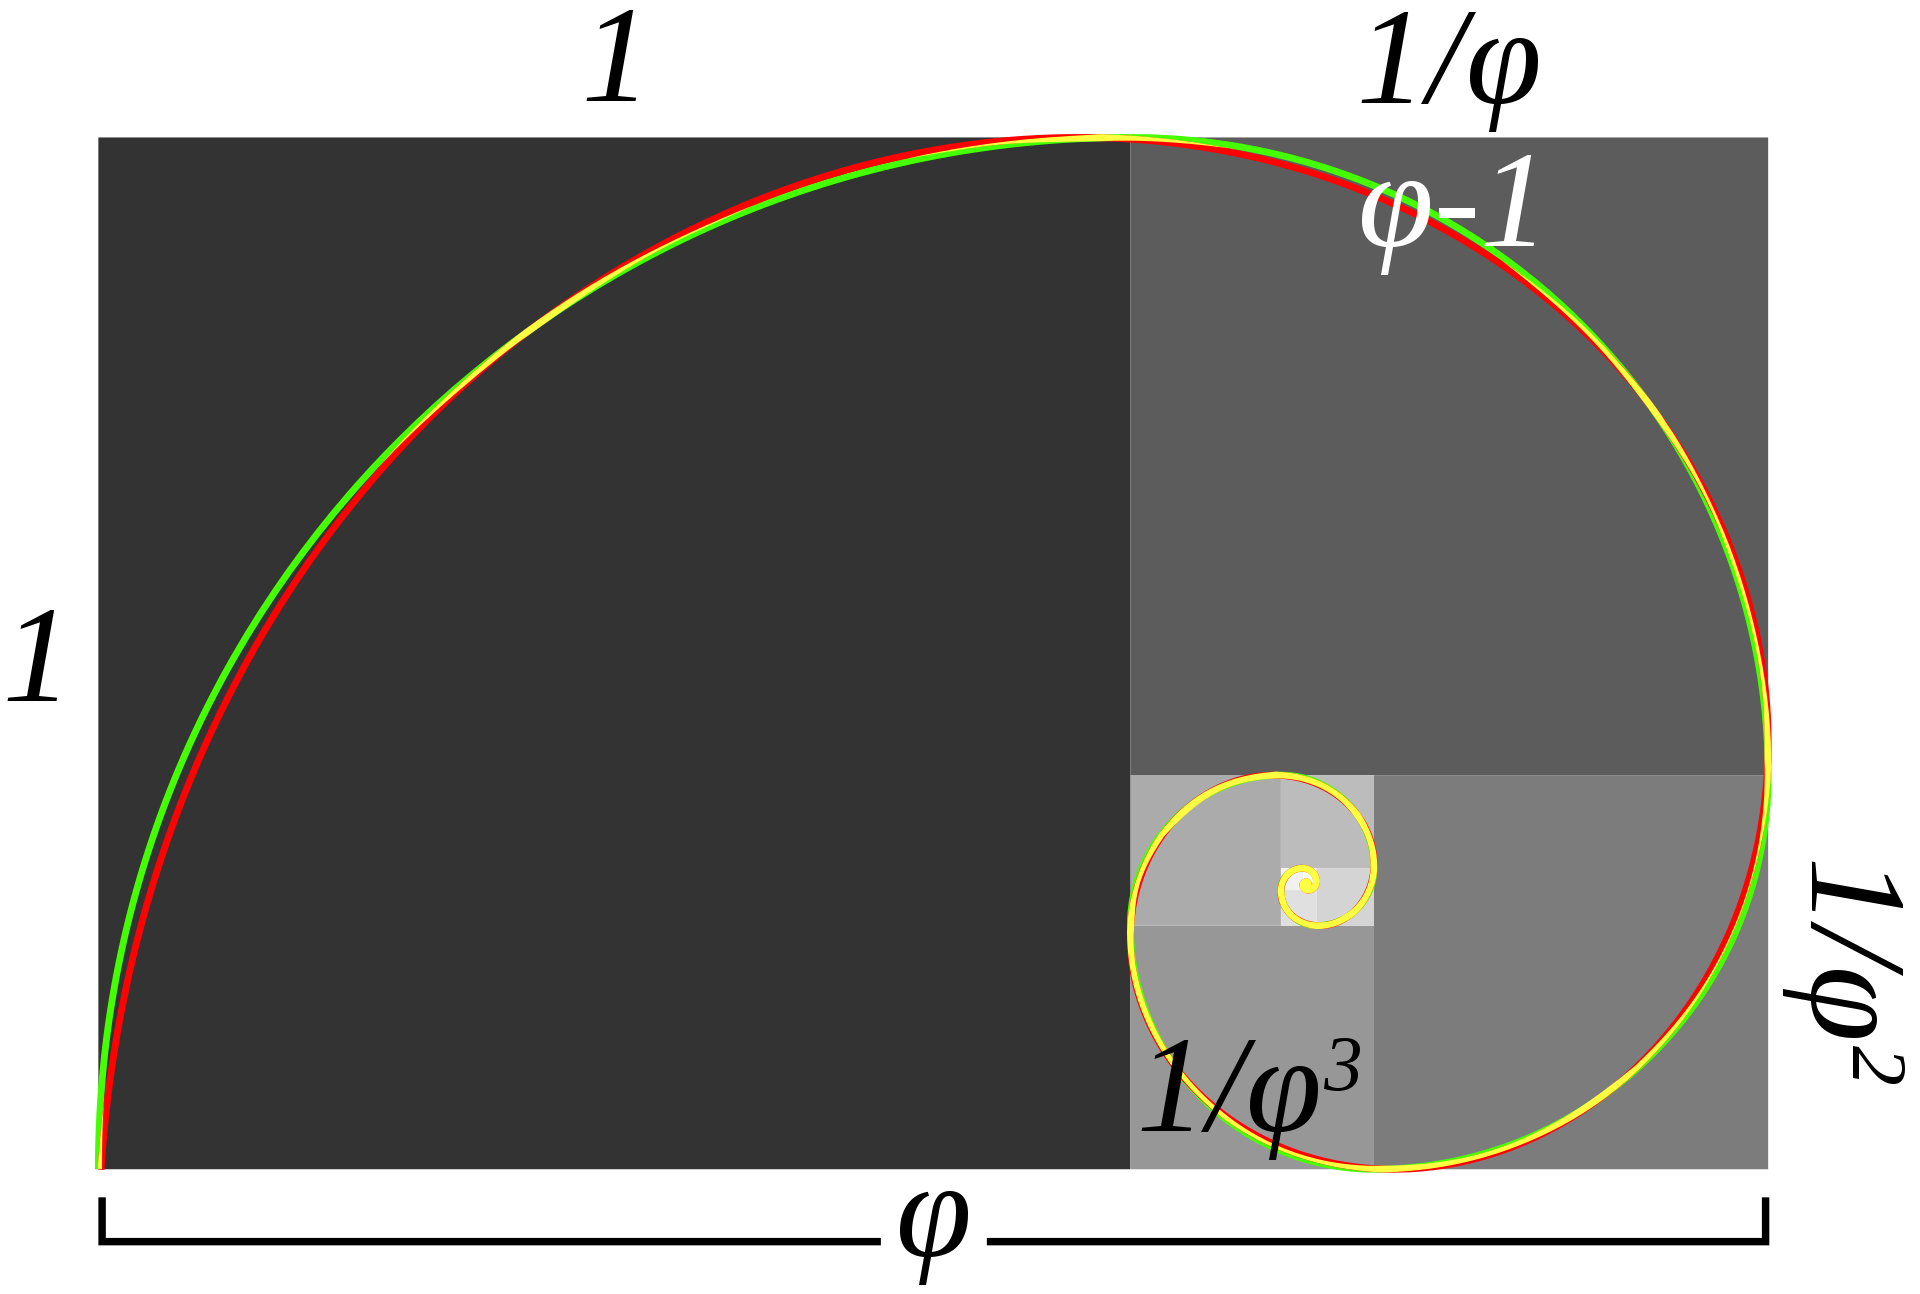
\includegraphics[height=0.25\textwidth, frame]{images/fake_real_log_spiral.png}}
        \hfill
        \subbottom[Спираль Фибоначчи\label{fig:spirals:b}]{%
            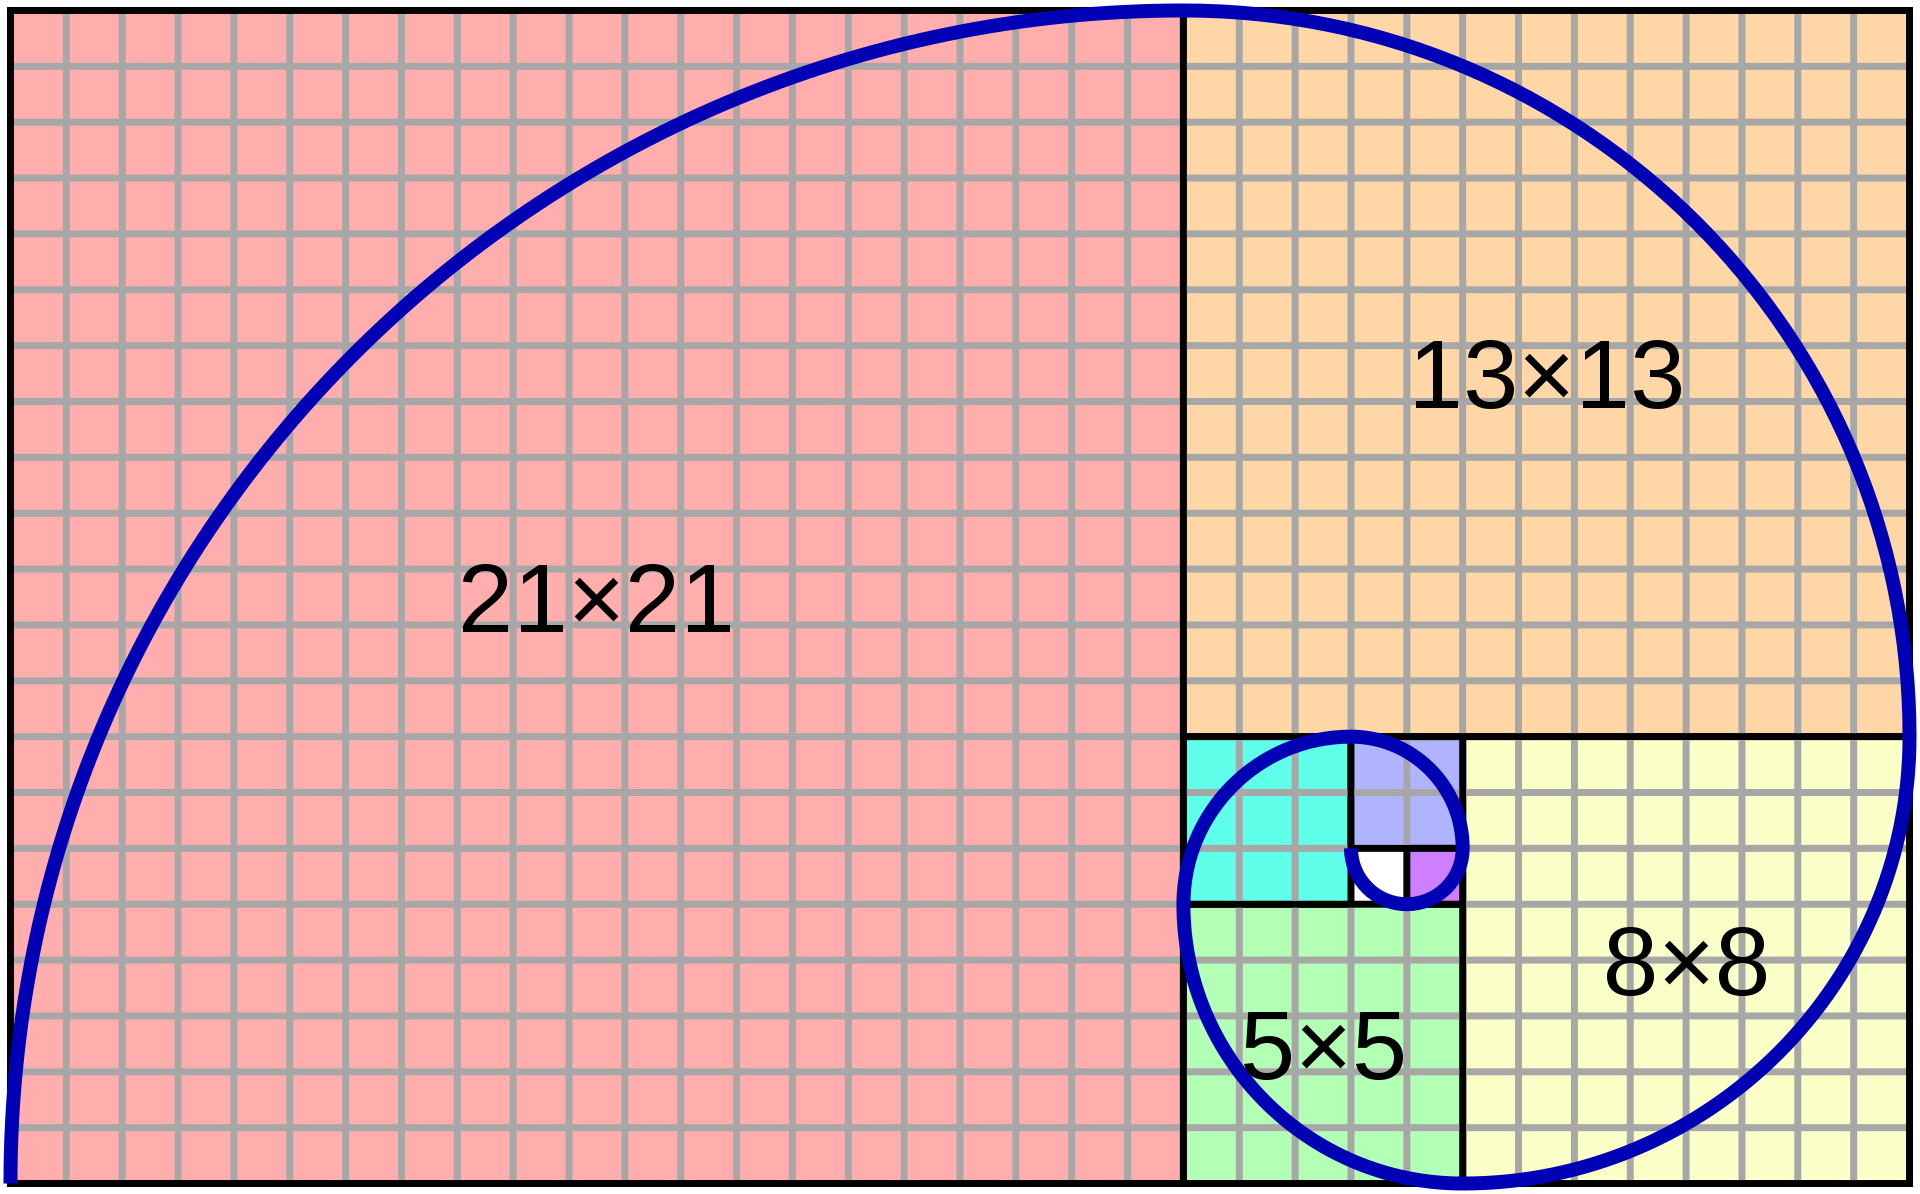
\includegraphics[height=0.25\textwidth]{images/fibonacci_spiral.png}}
        \hfill
    }
    \caption{Приближения золотой спирали}
    \label{fig:spirals}
\end{figure}

\item При~вписывании \emph{золотой спирали} в~последовательность вложенных друг в~друга золотых прямоугольников, она аппроксимируется спиралью, построенной по~методу Дюрера. Золотой прямоугольник можно разделить на~квадрат и подобный ему прямоугольник, его, в~свою очередь, разделить тем же образом, и продолжать этот процесс произвольное число раз. Если в~эти квадраты вписать соединенные между собой четвертинки окружностей, то получается спираль, изображённая на~рисунке~\ref{fig:spirals:a} зелёным цветом.

\smallskip

Спираль Фибоначчи строится подобно вышеописанной спирали, за~исключением того, что начинают с~прямоугольника из~двух квадратов и добавляют потом к~большей стороне прямоугольника квадрат такой же длины. Поскольку отношение между соседними числами Фибоначчи стремится к~золотой пропорции, спираль всё больше приближается к~золотой спирали по~мере добавления квадратов.

\begin{figure}[ht]
    {\centering
        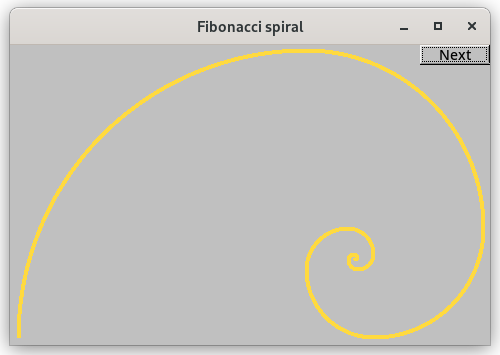
\includegraphics[height=0.25\textwidth]{images/fibonacci_spiral_draw.png}
        \hspace{1.5cm}
        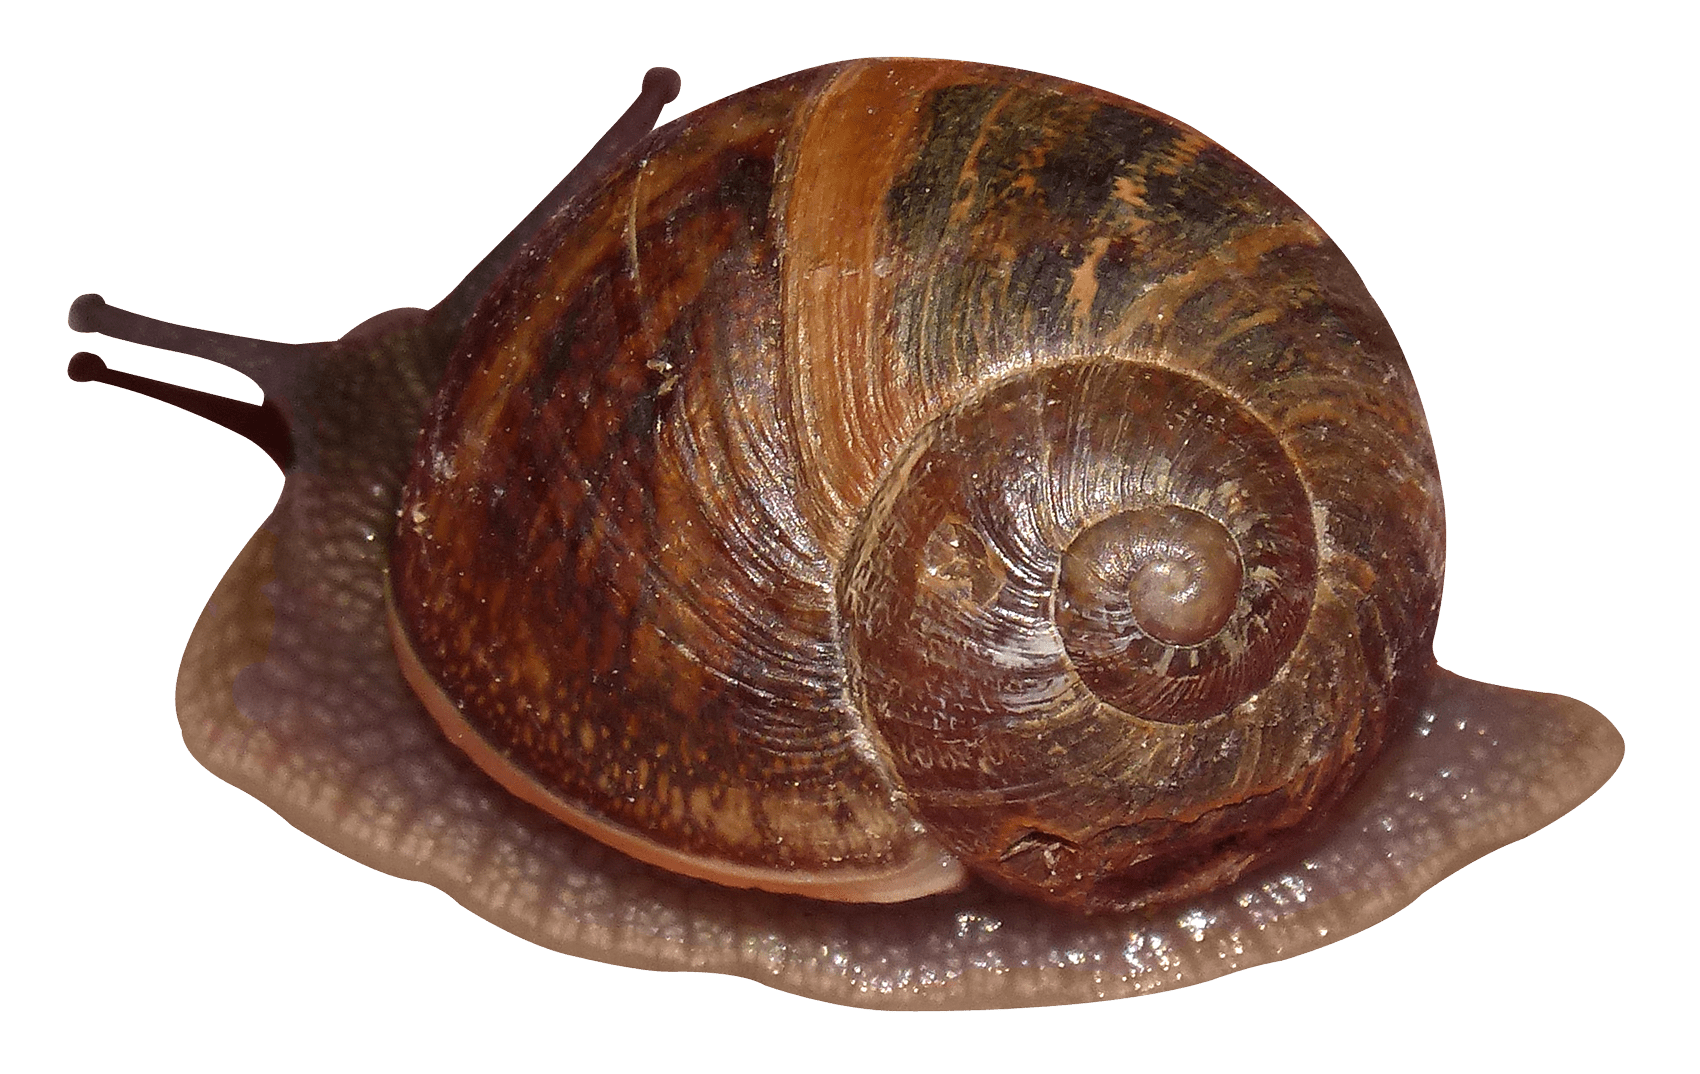
\includegraphics[height=0.25\textwidth]{images/snail.png}

    }
    \caption{Спираль Фибоначчи}
    \label{fig:fibonaccispiral}
\end{figure}

Нарисуйте спираль Фибоначчи, используя класс \code{Arc}, который был создан в~одном из~упражнений.
\end{exercise}
